\chapter{Analysis and Discussion of Model Results} % (fold)
\label{cha:analysis_of_model_results}
In the study of evolutionary dynamics there exists the concept of an stable equilibrium. The organisms in such a situation may not all represent the ``best fit'' mechanism for coping with a particular ecological niche, but at the same time none are sufficiently better off than the others that they will dominate the population. If organisms polymerizing nucleotides in a $3'\to5'$ direction represented a stable equilibrium with organisms polymerizing in a $5'\to3'$ direction, then it would be expected that organisms exhibiting such a trait should be found in nature. On the other hand, if $3'\to5'$ polymerization is a loosing strategy when in competition with $5'\to3'$ polymerization, the lack of modern $3'\to5'$ polymerizing organisms would be an expected consequence of Darwinian evolution.

When modeling the competition between organisms with a $5'\to3'$ polymerase and organisms with a $3'\to5'$ polymerase, this is an important aspect of modern evolutionary theory to keep in mind. It is not sufficient to show that polymerizing nucleotides in a $5'\to3'$ direction is better fit than, or produces organisms which reproduce faster than polymerizing nucleotides in a $3'\to5'$ direction. Rather, to discriminate between the possibility that the modern ubiquity of $5'\to3'$ polymerases is the result of a founder effect versus being a consequence of natural selection, we need to show that $3'\to5'$ polymerizing organisms cannot exist in a stable equilibrium. It is with this in mind that the model presented here was constructed.

In constructing this model, a number of explicit and implicit assumptions were made. The first, and perhaps largest, assumption is that polymerizing nucleotides to create new nucleic acid polymers by adding nucleotide triphosphates to the $5'$ end of the growing chain is physically possible. As there are no known polymerase enzymes which carry out the polymerization reaction in a $3'\to5'$ direction, it is impossible to say with certainty that such polymerases might exist. However, based on the nature of the active site chemistry of nucleotide polymerases, there is also no reason to believe that such $3'\to5'$ polymerases are not possible, beyond the fact that such polymerases do not currently exist. For this reason, we are comfortable with this assumption.

The second implicit assumption made in constructing this model is that the only viable building blocks for nucleic acid polymers are $5'$-triphosphate nucleotides. If nucleotides phosphorylated on their $3'$ oxygen could be used by a hypothetical $3'\to5'$ polymerase, then the chemistry of such a polymerase would not, qualitatively, be any different than that of a $5'\to3'$ polymerase working with $5'$-triphosphate nucleotides. That is, in the case that a $3'\to5'$ polymerase could work with a $3'$-triphosphate nucleotide, then the activated triphosphate moiety would reside on the incoming nucleotide, instead of on the growing chain, in the same way that the triphosphate moiety is found on the incoming $5'$-triphosphate nucleotide used by $5'\to3'$ polymerases.

We can discount the possibility of $3'$-triphosphate nucleotides as raw material for a polymerase reaction for a number of reasons. If, in keeping with current scientific consensus, ribonucleic acids represent the more ancient form of nucleotides and the $2'$-deoxyribonucleic acids are a more recent invention of biology, then a potential $3'$-triphosphate nucleotide would have its triphosphate group attached on a carbon adjacent to a free hydroxyl. The free $2'$-hydroxyl group of ribonucleic acids is known to polymerize hydrolysis reactions in a number of ribozymes, so it would not be unreasonable to assume that the $2'$-hydroxyl would also catalyze a hydrolysis of the triphosphate group on a $3'$-triphosphate nucleotide. This would serve to significantly restrict the available primordial pool of $3'$-triphosphate nucleotides as compared to $5'$-triphosphate nucleotides, whose adjacent carbon's oxygen would normally be incorporated in the formation of the furanose ring. Indeed, it has been shown that ribose-$3'$-phosphate decomposes more readily under mild acid conditions than ribose-$5'$-phosphate.

The remaining assumptions made are the various explicit assumptions required for construction of the model itself as described in chapter~\ref{cha:design_of_the_polymerase_evolution_model}. Of these, the two most important are the assumption that the dynamics of spontaneous nucleotide hydrolysis occur on a time-scale commiserate with the time-scale of nucleotide incorporation and the assumption of a geometry-based discrimination mechanism for incorrect nucleotide incorporation by the polymerase. As for the first of these two, we can surmise that the time-scale for spontaneous nucleotide hydrolysis cannot be significantly smaller than the time-scale for nucleotide incorporation, for if it were then nucleotide polymerization would, in effect, be impossible. If the time-scale were much larger, this would be the equivalent of removing a constant factor from the calculation for the probability that nucleotide inactivation occurs during polymerization. The effect of such an adjustment would be largely quantitative, raising the simulation temperature at which the effects reported would be observed. As for the assumption of geometry-based discrimination by the polymerase, the same experiments reported herein were reproduced without said mechanism incorporated in the model (data not shown). The only difference in the results from these experiments was that the viability of reverse polymerizing organisms at the highest temperatures (see figure~\ref{fig:strict_num}) was not observed.

A note should be made on the significance of the simulation temperature used in the model. If we take the expression used in the model for the temperature dependence of the equilibrium between the polymerase-template-nucleotide complex for the correct nucleotide, the free polymerase-template complex, and the polymerase-template-nucleotide complex for the incorrect nucleotide: $e^{-\frac{1}{t}}$, and compare it to the experimentally determined value of $5 \frac{kcal}{mol}$ for the $\Delta\Delta G$ of this system, we can calculate the real temperature corresponding to each simulation temperature with the expression\[
	T = t \frac{5\frac{kcal}{mol}}{R}
\]
This gives us a real temperature of $-22^\circ \rm{C}$ for a simulation temperature of 0.10 and a real temperature of $1200^\circ \rm{C}$ for a simulation temperature of 0.60. Obviously this range of temperatures is unreasonably large for life, even when accounting for aqueous environments with high salinity or at large pressures.

As mentioned in the introduction, every effort was made when designing this model to remain faithful to the realities of the biochemical processes that a nucleotide polymerase must carry out. That said, a number of confounding factors limit the applicability of the precise quantitative temperature values used in the simulations to understanding real biological processes. It has already been mentioned that the need to reduce the probability of spontaneous nucleotide hydrolysis by a constant factor to account for a difference in time-scales would effect the absolute temperature values at which various simulation outcomes are observed. The same sort of constant factor consideration would, potentially, also need to be made to account for a difference between the precise effect of geometry-based discrimination of real nucleotide polymerases and the model values.

The primary model values impacted by simulation temperature are those for the equilibrium describing the incorporation of correct versus incorrect nucleotides during nucleic acid synthesis, and the equilibrium between active and inactive nucleotides. The chemical phenomena described by these values, however, are subject to more influences than just temperature. For example, it is well documented that the energy associated with a correct nucleotide base-pairing is heavily influenced by the dielectric constant of the solvent and the concentration of nucleic acid counter-ions. The equilibrium of nucleotide triphosphates would, likewise, be subject to influence by effects of nucleotide concentration and pH. Thus, the value of simulation temperature can be thought of as a stand in for a number of thermodynamic factors that might influence the biochemical processes involved in the model processes. Therefore, the primary utility of the simulation temperature is in revealing the collected influence of thermodynamics on the system.

Before we consider these influences, let us look at the results of the initial experiments performed with the model. In figure~\ref{fig:temp_incr_num}, we can see that the model fairly accurately captures the exponential growth phase that is empirically observed in nature. At lower simulation temperatures, the gradual leveling off to a stationary phase population plateau is not as clean as we might like. Particularly, there seems to be a under-damping of growth by the simulation's population based culling probability. Still, an informative comparison can be made between the growth rates of forward and reverse polymerizing organisms. At the lower simulation temperatures of 0.10 and 0.30, there is effectively no difference between the two categories of organism. As the temperature is increased successively to 0.40, 0.50, and 0.60, the difference in population between the forward and reverse polymerizing organisms at each simulation time step becomes successively greater, to the point where, at a simulation temperature of 0.60, there is effectively no growth of the reverse polymerizing organisms. This difference in growth is expected due to the extra penalty suffered by reverse polymerizing organisms when a nucleotide triphosphate spontaneously hydrolyzes.

Remember that in these first experiments there is no competition between forward and reverse organisms. Each sort of organism is being allowed to grow in isolation. This explains why, in figure~\ref{fig:temp_incr_rate} there is essentially no difference in the evolution of polymerase rates between the two. When growing in isolation, the only evolutionary pressures present are the deleterious effects of too many polymerization errors and density dependent culling, and these two factors will be experienced identically by either forward or reverse polymerizing organisms.

As we begin to put the organisms in competition with each other, figure~\ref{fig:cluster_growth_rate} reveals that, at higher temperatures, the evolution of the polymerase rates of the forward and reverse polymerizing organisms begin to diverge from each other. At the lower temperatures of 0.10 and 0.30, there is still effectively no difference in the relative polymerase rates of the forward and reverse organisms. It is interesting to note, though, that the absolute value of polymerase rate for the populations in competition is lower than that of the populations in isolation at these temperatures. Another way of stating this is that the overall fitness of the organisms in the environment is reduced when they are in competition. This is an expected outcome based on current evolutionary dynamics theory.

At the higher temperatures, the average polymerase rate of the reverse polymerizing organisms begins to drop off as their population numbers, as seen in figure~\ref{fig:cluster_growth_num}, begin to drop off. This drop is not, however, indicative of a reduction in the fitness of the reverse polymerizing organisms. Rather, as the reverse polymerizing organisms are gradually outcompeted by the forward polymerizing organisms their number is reduced. Since the only mechanism in the model for removing organisms from the population is the density dependent random culling, which members of the reverse polymerizing organism population will be removed is likewise random. Since the organisms with a faster polymerase rate will reproduce more rapidly, they will be present in greater number, and therefore will be more likely to be removed from the environment first. In other words, the rate of the decrease in average polymerase rate of the reverse polymerizing organisms can be seen as a proxy measure for the rate at which the forward polymerizing organisms are preferentially occupying the available capacity in the environment created when a reverse polymerizing organism is culled.

Based on this result, what seems to be the most interesting aspect of the simulation, then, is how available capacity is occupied by one or the other sort of organism following a random death. That is, competition between the organisms when the environment is at capacity will probably reveal more about the comparative fitness of the two polymerase strategies than following exponential growth from a small starting population. It is also worth noting that, especially at the higher temperatures, starting with a small population is not the best strategy for comparing forward and reverse polymerizing organisms since both sorts of organism experience significant hardship growing beyond their starting population. Indeed, while the population of forward polymerizing organisms at a simulation temperature of 0.60 appears to remain remarkably stable at approximately 500, what this actually represents is that in the 10 repetitions of this simulation carried out, there was a 50/50 chance of the initial population of forward polymerizing organisms surviving at all (and those that did maintained a nearly full environment of 1000 organisms).

It was for these reasons that the last set of experiments, starting with an already full environment, were performed. The justification in starting with an evenly split population relies on another aspect of stable evolutionary equilibria. Namely, if there is a stable equilibrium between forward and reverse polymerizing organisms, then any starting population containing these two types will converge on the equilibrium ratio of one to the other. If, on the other hand, one or the other sort of organism is dominant, then even a small starting population of the dominant organism will eventually overcome the other. This implies that any ratio of forward and reverse polymerizing organisms in the starting population would be valid, and then the choice of an even split is made to reduce the possibility of an early random fluctuation causing an unrealistic culling of one or the other sort of organism.

Looking at figure~\ref{fig:strict_rate}, we can see that the dynamics of the evolution of polymerase rate at each temperature in the case of starting with a full environment are similar to those of starting with a small seed population. Now, though, we can look at figure~\ref{fig:strict_num} and see that, as we hypothesized, the decrease in rate does correspond to the inability of the reverse polymerizing organisms to sustain their population in the face of competition from forward polymerizing organisms at simulation temperatures of 0.40 and 0.50. Furthermore, at a simulation temperature of 0.50, where the average polymerase rate of the reverse polymerizing organisms drops off most rapidly, we can see that the decrease in population of the reverse polymerizing organisms seems to only be limited by the rate at which the forward polymerizing organisms can reproduce and occupy the available capacity freed by culling. In other words, at this temperature it appears as if nearly every culled organism, forward or reverse, is replaced by a forward polymerizing organism. This matches the expectation for a situation in which one organism is strictly dominant.

Starting with a full environment reveals a few other interesting aspects of the model. Focusing on the early time points in the simulations in figure~\ref{fig:strict_rate}, we can now clearly see that the evolution of polymerase rate of the reverse polymerizing organisms lags that of the forward polymerizing organisms at every temperature. At the lower simulation temperatures of 0.10 and 0.30, the reverse polymerizing organisms eventually catch up with the forward polymerizing organisms to set up a stable equilibrium as revealed by the stable populations of forward and reverse polymerizing organisms at later points in the simulations at these temperatures (figure~\ref{fig:strict_num}). The one exception to this rule appears at a simulation temperature of 0.60.

Curiously, at a simulation temperature of 0.60, the reverse polymerizing organisms are, again, able to set up a stable equilibrium with the forward polymerizing organisms. This aspect of the simulation could not have been predicted by the results from starting with a small seed population. In figure~\ref{fig:cluster_growth_num} at a simulation temperature of 0.60, the reverse polymerizing organisms never get a chance to build up any significant population. Yet, starting with a full environment, we can see that these organisms survive rather stably in competition with the forward polymerizing organisms. In this particular case, what we are observing is not any increase in fitness of the reverse polymerizing organisms, but rather a steeper decrease in the fitness of the forward polymerizing organisms. This is further emphasized by the fact that, unlike the lower simulation temperatures of 0.10 and 0.30 where the reverse polymerizing organisms are only able to achieve a stable equilibrium once they evolve their polymerase rates to match those of the forward polymerizing organisms, at a simulation temperature of 0.60 the reverse polymerizing organisms have a polymerase rate significantly lower than that of the forward polymerizing organisms once stable equilibrium is achieved.

\begin{figure}[ht]
	\centering
		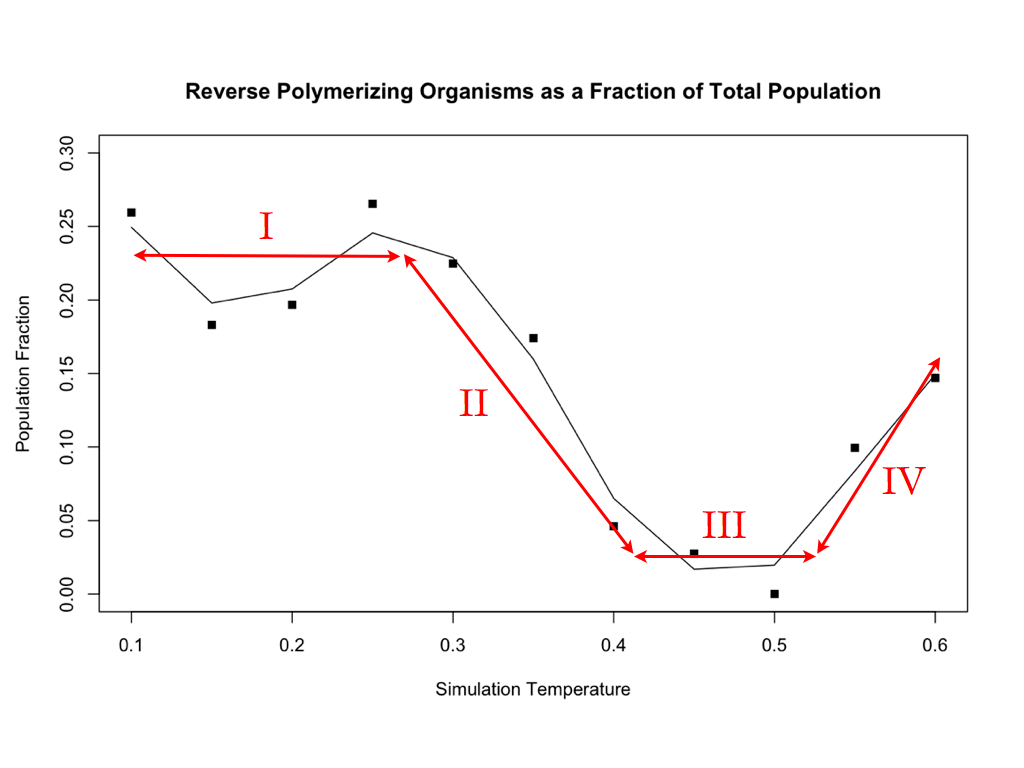
\includegraphics[width=\textwidth]{competition_regimes}
	\caption{\textbf{Competition Regimes.} The average population fraction of reverse polymerizing organisms over the last 25000 simulation time steps from figure~\ref{fig:strict_num_rev} is plotted against simulation temperature. The black line is a smoothed spline constructed from the data, and the red arrows highlight the four competition regimes observed: I. Stable Low-Temperature Equilibrium, II. Weak Evolutionarily Stable Strategy, III. Evolutionarily Stable Strategy, IV. Stable High-Temperature Equilibrium.}
	\label{fig:competition_regimes}
\end{figure}

It seems, then, as if there are multiple regimes of competition that the forward and reverse polymerizing organisms go through as simulation temperature is raised. We can see that this is the case by looking at a larger set of temperatures in figure~\ref{fig:strict_num_rev}. This figure reveals at least four competition regimes (see figure~\ref{fig:competition_regimes}). The first is a stable equilibrium between the forward and reverse polymerizing organisms that occurs at low temperatures where the reverse polymerizing organisms have a chance to evolve their polymerases to match those of the forward polymerizing organisms before they are outcompeted. The second regime resembles a weak evolutionarily stable strategy. Such a situation is characterized by one organism which is able to dominate over another, but only through a process of selection. That is, over time, selection will favor the forward polymerizing organisms at this temperature. The third regime resembles a pure evolutionarily stable strategy, one where the dominant organism is immune to invasion by the lesser organism. This is where the forward polymerizing organisms grow to occupy any vacancies left by dying reverse polymerizing organisms. The reverse polymerizing organisms aren't even given the chance to compete for these spots. The final regime represents the unexpected high-temperature stable equilibrium. This is the case we saw where the forward and reverse polymerizing organisms are able to co-exist while still having very different polymerase rates. In this regime, rate of reproduction is no longer the dominant selective force. Rather, the high rate of mutation, and the ability of the organisms to reproduce in the face of such, becomes more important.

To answer the question first posed, it is conceivable that the $5'\to3'$ nucleotide polymerases which exist, exclusively, in nature today were the result of a Darwinian competition between these and the alternative, $3'\to5'$ nucleotide polymerases. We cannot say for sure that this is the case without having a firmer grasp on the specific values for a number of model parameters, and the temperature at which life first originated. The possibility that the success of $5'\to3'$ nucleotide polymerases was the consequence of a founder effect still remains. However, by attempting to model this evolutionary process, we have come upon a potentially more interesting result. We have, as illustrated in figure~\ref{fig:competition_regimes}, a model system where thermodynamic influences may determine the nature of the competition between two alternatives.
% chapter analysis_of_model_results (end)